\documentclass[a4paper, 6pt, landscape]{scrartcl}

\usepackage[german]{babel} %choose your language
\usepackage[landscape, margin=1cm]{geometry}
\usepackage[utf8]{inputenc}
\usepackage[dvipsnames]{xcolor}
\usepackage{amscd, amsmath, amssymb, blindtext, empheq, enumitem, multicol, parskip}
\usepackage{graphicx}
\usepackage{tikz}
\usepackage{esint}
\usepackage{wrapfig}
\usepackage{setspace}
\usepackage{trfsigns}

% make document compact
\usepackage[compact]{titlesec}
\titlespacing{\section}{0pt}{*0}{*0}
\titlespacing{\subsection}{0pt}{*0}{*0}
\titlespacing{\subsubsection}{0pt}{*0}{*0}

\parindent 0pt
\pagestyle{empty}
\setlength{\unitlength}{1cm}
\setlist{leftmargin = *}

% Set the color of your style
% Avaiable are: Apricot, Aquamarine, Bittersweet, Black, Blue, blue, BlueGreen, BlueViolet, BrickRed, Brown, BurntOrange, CadetBlue, CarnationPink, Cerulean, CornflowerBlue, Cyan, Dandelion, DarkOrchid, Emerald, ForestGreen, Fuchsia, Goldenrod, Gray, Green, GreenYellow, JungleGreen, Lavender, ... (more at: http://en.wikibooks.org/wiki/LaTeX/Colors)
\def\StyleColor{Yellow}

\DeclareMathOperator{\rot}{rot}
\DeclareMathOperator{\divg}{div}


% define some colors
\usepackage{color}
\definecolor{section}{RGB}{90,110,255}
\definecolor{subsection}{RGB}{160,180,255}
\definecolor{subsubsection}{RGB}{220,230,255}
\definecolor{titletext}{RGB}{0,0,0}
\definecolor{formula}{RGB}{220,230,255}

% section color box
\setkomafont{section}{\mysection}
\newcommand{\mysection}[1]{%
    \Large\sf\bf%
    \setlength{\fboxsep}{0cm}%already boxed
    \colorbox{section}{%
        \begin{minipage}{\linewidth}%
            \vspace*{2pt}%Space before
            \leftskip2pt %Space left
            \rightskip\leftskip %Space right
            {\color{titletext} #1}
            \vspace*{1pt}%Space after
        \end{minipage}%
    }}
%subsection color box
\setkomafont{subsection}{\mysubsection}
\newcommand{\mysubsection}[1]{%
    \normalsize \sf\bf%
    \setlength{\fboxsep}{0cm}%already boxed
    \colorbox{subsection}{%
        \begin{minipage}{\linewidth}%
            \vspace*{2pt}%Space before
            \leftskip2pt %Space left
            \rightskip\leftskip %Space right
            {\color{titletext} #1}
            \vspace*{1pt}%Space after
        \end{minipage}%
    }}
    
%subsection color box
\setkomafont{subsubsection}{\mysubsubsection}
\newcommand{\mysubsubsection}[1]{%
    \normalsize \sf\bf%
    \setlength{\fboxsep}{0cm}%already boxed
    \colorbox{subsubsection}{%
        \begin{minipage}{\linewidth}%
            \vspace*{2pt}%Space before
            \leftskip2pt %Space left
            \rightskip\leftskip %Space right
            {\color{titletext} #1}
            \vspace*{1pt}%Space after
        \end{minipage}%
    }}    
%subsection color box
\title{Zusammenfassung NuS I D-ITET}
\author{Manuel Meier}
\date{\today}


\newcommand{\dis}[1]{\hspace{#1cm}}
    
% equation box        
\newcommand{\eqbox}[1]{\fcolorbox{section}{formula}{\hspace{0.5em}$\displaystyle#1$\hspace{0.5em}}}

%macro for vectors 
%\newcommand{\vect}[1]{\vec{#1}}
\newcommand{\vect}[1]{\boldsymbol{#1}}

%\renewcommand{\familydefault}{cmss}
\DeclareSymbolFont{letters}{OML}{ztmcm}{m}{it}
\DeclareSymbolFontAlphabet{\mathnormal}{letters}

%\everymath{\displaystyle}  %bigger equations
\begin{document}
%\setcounter{secnumdepth}{0} %no enumeration of sections
	\begin{multicols*}{4}
		\maketitle
			\section{Elektrostatik}
				\doublespacing			
				\begin{tabular}{llll}
					\textbf{Elementarladung} &$e  $&$ +1.602\cdot 10^{-19}$&$As$\\
					\textbf{Dielektrizitätskonst.}& $\varepsilon_0  $&$ 8.854\cdot 10^{-12}$&$\frac{As}{Vm}$\\
					\textbf{Magn. Permeabilität}& $\mu_0  $&$ 4\pi\cdot 10^{-7}$&$\frac{Vs}{Am}$\\
					\textbf{Ruhemasse Elektron}& $m_{0,e}  $&$ 9.1094\cdot 10^{-31}$&$kg$\\
					\textbf{Ruhemasse Proton} &$m_{0,p}  $&$ 1.6726\cdot 10^{-27}$&$kg$\\
					\textbf{Lichtgeschwindigkeit} &$c_{Vak.}  $&$ 2.99792\cdot 10^8$&$\frac{m}{s}$\\
				\end{tabular}
				
				Sinussatz: $\frac{a}{\sin \alpha} = \frac{b}{\sin \beta} = \frac{c}{\sin \gamma} = \frac{abc}{2A} = 2R$\\
Kosinussatz: $c^2 = a^2 + b^2 -2ab\cos \gamma$
				\singlespacing 				
				\subsection{Ladungsdichten}
				\begin{itemize}
					\item \textit{Linienladungsdichte:} $\lambda=\frac{dQ}{dl}=\left[\frac{As}{m}\right], Q=\int_l\lambda dl$
					\item \textit{Flächenladungsdichte:} $\sigma=\frac{dQ}{dA}=\left[\frac{As}{m^2}\right], Q=\iint_A\sigma dA$
					\item \textit{Raumladungsdichte:} $\rho=\frac{dQ}{dV}=\left[\frac{As}{m^3}\right],Q=\iiint_V\rho dV$
				\end{itemize}
				
				\subsection{Grundgrössen}
				\begin{itemize}
					\item \textbf{E-Feld einer Punktladung:} $\vec{E}=\frac{1}{4\pi\varepsilon_0}\frac{Q}{r^2} \quad [\frac{V}{m}]$
					\item \textbf{Kraft mehre. zweier Ladungen:} $\vec{F}=\frac{Q_1Q_2}{4\pi\varepsilon_0r^2}\vec{e_r} \quad [N]$
					\item \textbf{E-Feld Punktldgn:}
					$\vec{E}(\vec{r_p})=\frac{1}{4\pi\varepsilon_0}\cdot\sum_k\frac{Q_k}{|\vec{r_p}-\vec{r_k}|^2}\frac{\vec{r_p}-\vec{r_k}}{|\vec{r_p}-\vec{r_k}|}$
					\item \textbf{E-Feld $\infty$-langer Leiter:} $E=\frac{1}{2\pi\varepsilon_0}\frac{\lambda}{r_\bot}$
					\item \textbf{Spannung, Innen-/Aussenleiter:} $\vec{E}(\rho)=\frac{Q}{2\pi\varepsilon l}\frac{1}{\rho}\vec{e_{\rho}}$\\
					$\displaystyle{U=\int_{r_1}^{r_2}{\vec{E}(\rho)}d\vec{\rho}=\int_{r_1}^{r_2}{\frac{Q}{2\pi\cdot\varepsilon\cdot l}\frac{1}{\rho}}d\rho}=\frac{Q}{2\pi\cdot\varepsilon\cdot l}\ln{\left| \frac{r_2}{r_1} \right|}$\\
					\item \textbf{Leckstrom:}
					\\ $\displaystyle{I=\int_{0}^{2\pi}{\int_{0}^{l}{\vec{J}(\rho)\rho}dz}d\varphi=2\pi\kappa\rho
					 l E(\rho)}$  $\Rightarrow E(\rho)=\frac{I}{2\pi\kappa l}\frac{1}{\rho}$
					 \item \textbf{Elektr. Flussdichte }$\vec{D}(\vec{r})=\varepsilon_0\cdot\varepsilon_r\cdot\vec{E}(\vec{r})=\varepsilon\cdot\vec{E}(\vec{r})\quad [\frac{As}{m^2}]$
				\end{itemize}

				\subsubsection{Arbeit \& Potential (1-33)}
				$W_{P_1\rightarrow P_2}=-\int_{P_1}^{P_2}{\vec{F}\cdot}d\vec{s}$ \dis{0.5} weg-unabhängig\\
				$W_{e}=-Q\int_{P_1}^{P_2}{\vec{E}\cdot}d\vec{s}=Q\left(\varphi(P_2)-\varphi(P_1)\right)=-U_{12}Q$\\
				$\rightarrow [W]=Ws=J, [P]=\frac{J}{s}=W$\\ \\
				\textbf{Potential:}\\
				Oftmals $P_{ref}=\infty$\\
				$\varphi(P_1)=\frac{W(P_{ref}\rightarrow P_1)}{Q_1}=-\int_{P_{ref}}^{P_1}{\vec{E}\cdot}d\vec{s} \quad [V]$
				\subsubsection{Spannung}
				$U_{12}=\varphi(P_1)-\varphi(P_2)=\int_{P_1}^{P_2}{\vec{E}\cdot}d\vec{s}=\frac{W_{12}}{Q}$
				\subsection{Das Gauss'sche Gesetz (1-45)}
				\begin{center}
				\eqbox{\oint_A{\vec{D}(\vec{r})}d\vec{A} = \oint_A{\vec{e_r}D(r)}\vec{e_r}dA=Q}
				\end{center}
				
				E-Feldlinien von idealen Leitern, stehen senkrecht auf der Oberfläche.				
					


				
				
				
				
				\subsection{Kondensator (1-61)}
				\begin{center}
				\eqbox{C=\frac{Q}{U}=\frac{\varoiint_A{\vec{D}\cdot}d\vec{A}}{\int_s{\vec{E}\cdot}d\vec{s}}=\frac{\varoiint_A{\sigma}dA}{\int_s{\vec{E}\cdot}d\vec{s}} \quad [F]=[\frac{As}{V}]}\\
				\end{center}
				Einfache Kondensatorentladung: $U=U_0e^{\frac{-t}{RC}}$
				\begin{itemize}
					\item \textbf{Plattenkondensator:}\\
					$E=\frac{D}{\varepsilon}=\frac{\sigma}{\varepsilon}=\frac{Q}{\varepsilon A},$ \dis{0.2} $U=Ed\rightarrow C=\frac{Q}{U}=\frac{\varepsilon A}{d}$\\ \\
					Das Feld einer Platte ist $E/2$
					\item \textbf{Kugel(schalen)kondensator: (1-62)(1-73)}\\
					\mbox{$U_{ab}=\int \limits_{r_i}^{r_a} \vec{E}\cdot d \vec{s} = \frac{Q}{4\pi\varepsilon}\int\limits_{r_i}^{r_a}{\frac{1}{r^2}}dr=\frac{Q}{4\pi\varepsilon}\frac{r_a-r_i}{r_ar_i}=\frac{Q}{C}\rightarrow C=4\pi\varepsilon\frac{r_ir_a}{r_a-r_i}$}
					\item \textbf{Vielschichtenkondensator aus n Platten:}\\
					$C_{ges}=(2n-1)C$
					\item \textbf{Drehkondensator (1-68)}\\
					$C_{ges}=(2n-1)\frac{\varepsilon A}{d}=(2n-1)\frac{\varepsilon}{d}\frac{\alpha}{2\pi}(\pi r_{\alpha}^2-\pi r_{i}^2)$\\ \\
					Für unendlich dünne Platten: $D=\sigma/2$
				\end{itemize}
				\subsection{Energie im E-Feld (1-70)(1-72)}
				\begin{center}
				\eqbox{W_e=\frac{1}{2}\frac{Q^2}{C}=\frac{1}{2}QU=\frac{1}{2}CU^2=\iiint_V{\frac{1}{2}\vec{E}\cdot\vec{D}}dV}
				\end{center}
			\section{Elektr., stationäres Strömungsfeld}
				\subsection{Strom}
				$\displaystyle{I=\frac{dQ}{dt}=\iint_A{\vec{J}\cdot}d\vec{A},}$ \dis{0.2} $[I]=A,$ \dis{0.2} $\displaystyle{J=\frac{dI}{dA},}$ \dis{0.2} $\displaystyle{[J]=\frac{A}{m^2}}$\\
				Stat. Strömungsfeld, wenn $I$ konst.: $\varoiint_{A}{\vec{J}\cdot}d\vec{A} = 0$ (1-86)\\
				\begin{itemize}
					\item \textbf{Spezifische Leitfähigkeit:}\\
					Driftgeschw. $\vec{v}_{Drift}=-\mu_e\vec{E}$ wobei $\mu_e=$ "Beweglichkeit"\\
					$\vec{J}=\vec{V}_{Drift}\rho=\underbrace{-\rho\mu_e}_\kappa\vec{E},$ \dis{0.2} $\kappa=$spez.Leitf.,
					$[\kappa]=\frac{A}{Vm}=\frac{1}{\Omega m}$
					\item \textbf{Spezifischer Widerstand:} $\rho_R=\frac{1}{\kappa},$ $[\rho_R]=\Omega m=\frac{Vm}{A}$
					\item \textbf{Temperaturabhängigkeit:}\\
					$\rho_R(T)=\rho_{R,20^\circ C}\left(1+\alpha(T-20^\circ C)\right)$
					\item \textbf{Ohmsches Gesetzt:} \eqbox{U=R\cdot I}, $[R]=\frac{V}{A}=\Omega$\\
					$\vec{J}=\kappa\vec{E},$\dis{0.2} $R=\frac{U}{I}=\frac{l}{\kappa A}=\frac{\rho_R l}{A}=\frac{\int_S{\vec{E}\cdot}d\vec{s}}{\kappa\iint_A{\vec{E}\cdot}d\vec{A}}$
					\item \textbf{Leitwert:} \eqbox{G=\frac{1}{R}} $[G]=S$ (Siemens)
				\end{itemize}
				\subsection{Sprungstellen bei Materialübergängen (1-99)}
				\begin{itemize}
					\item \textit{Normalkomponenten.:} \eqbox{J_{n1=J_{n2}}},\eqbox{\kappa_1E_{n1}=\kappa_2E_{n2}}\\
					Die Normalkomponente der Stromdichte ist stetig.
					\item \textit{Tangentialkomp.:} \eqbox{E_{t1}=E_{t2}},\eqbox{\frac{J_{t1}}{J_{t2}}=\frac{\kappa_1}{\kappa_2}}\\
					Die Tangentialkomponente des E-Feldes ist stetig.
				\end{itemize}
				\subsection{Energie und Leistung (1-102)}
				$\displaystyle{W_e=\int_{0}^{t}{P(\tau)}d\tau}$ und $P(t)=\frac{dW_e}{dt}$\\$P=UI=I^2R=U^2/R$\\
				\textbf{Verlustleistungsdichte:} $p_V=\frac{dP}{dV}=\vec{E}\cdot\vec{J}$\\
				$P=\iiint_V{p_V}dV=\iiint_V{\vec{E}\cdot\vec{J}}dV$
			\section{DC-Netzwerke}
				\subsection{Spannungs- und Stromquellen}
				\begin{itemize}
					\item \textbf{Ideale Quellen:}\\
					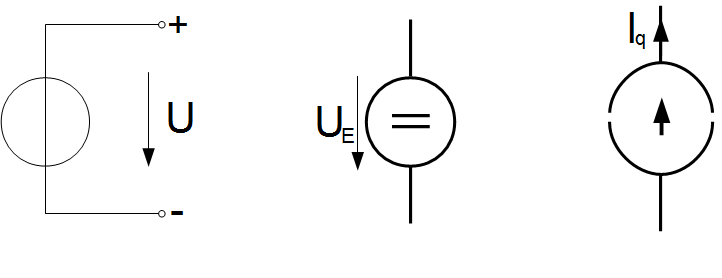
\includegraphics[scale=0.2]{source/quellen.png}
					$\rightarrow$ Keine Verlustleistung
					%\item \textbf{Leistung:} $P=UI=RI^2=\frac{U^2}{R}$
					\item \textbf{Reale Stromquelle} Leerlaufspannung: $U_0=R_i\cdot I_0$
					\item \textbf{Reale Spannungsquelle} Kurzschlussstrom: $I_K=\frac{U_0}{R_i}$
					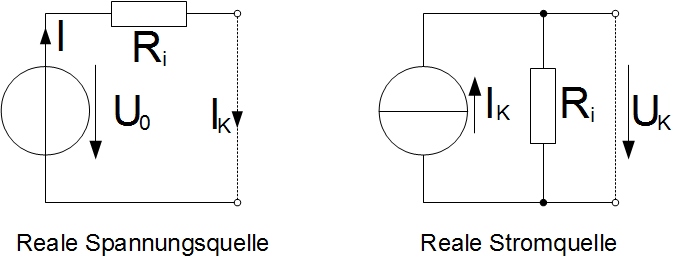
\includegraphics[scale=0.25]{source/realeQuellen.png}\\
					\textit{Umwandlung:} $_{[U-Quelle]}\,U_0=R_i\cdot I_0 \, _{[I-Quelle]}$
					\item \textbf{Kirchhoff'sche Maschenregel:} $\sum_{Masche}U_k=0$
					\item \textbf{Kirchhoff'sche Knotenregel:} $\sum_{Knoten}I_k=0$
					\item \textbf{Leistungsanpassung}\\
				Die Leistung wird maximiert, wenn gilt: \eqbox{R_L=R_i}
				\end{itemize}
				
				\textbf{Wechselwirkung Quelle $\Leftrightarrow$ Verbraucher}
				\begin{itemize}
					\item Gleichmässige Energieabgabe ist nur bei identischen Quellen möglich.
					\item Leistungsabgabe von zusammengeschalteten Spannungsquellen ist unterschiedlich, wenn sie über versch. $R_i$ oder $U_L$ verfügen.
					\item Quellen können zu \textit{Verbrauchern} werden.			
				\end{itemize}
				
				\subsection{Einfache Netzwerkberechnungen}
				\begin{tabular}{ll}
					\textbf{[R] Seriell:} &$R_{ges}=\sum\limits_{k=1}^{n}{R_k}$\\
					\textbf{[R] Parallel:} &$\frac{1}{R_{ges}}=\sum\limits_{k=1}^{n}{\frac{1}{R_k}}$ \quad $n=2\rightarrow R_{ges}=\frac{R_1R_2}{R_1+R_2}$\\
					\textbf{[C] Seriell:} &$\frac{1}{C_{ges}}=\sum\limits_{k=1}^{n}{\frac{1}{C_k}}$ \quad $n=2\rightarrow C_{ges}=\frac{C_1C_2}{C_1+C_2}$\\
					\textbf{[C] Parallel:} &$C_{ges}=\sum\limits_{k=1}^{n}{C_k}$\\
					\textbf{[L] Seriell:} &$L_{ges}=\sum\limits_{k=1}^{n}{L_k}$\\
					\textbf{[L] Parallel:} &$\frac{1}{L_{ges}}=\sum\limits_{k=1}^{n}{\frac{1}{L_k}}$ \quad $n=2\rightarrow L_{ges}=\frac{L_1L_2}{L_1+L_2}$				
				\end{tabular}

				\subsection{Spannungs-/Stromteiler}
				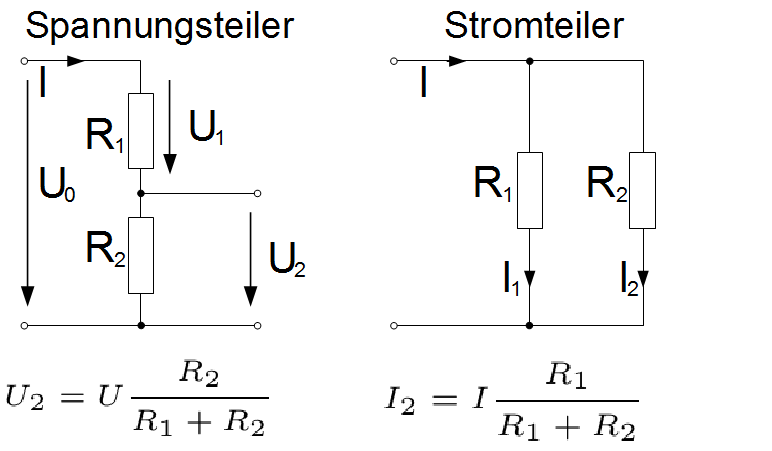
\includegraphics[scale=0.24]{source/teiler.png}\\\\
				\textbf{Belasteter Spannungsteiler:}\\
				$$R_{2}'=\frac{R_2R_L}{R_2+R_L}\rightarrow \frac{U_2}{U}=\frac{R_{2}'}{R_1+R_{2}'}=\frac{R_2R_L}{R_1(R_2+R_L)+R_2R_L}$$

				\subsection{Wirkungsgrad}
				$$\eta=\frac{P_L}{P_{ges}}\cdot 100\%=\frac{I^2R_L}{I^2(R_i+R_L)}\cdot 100\%=\frac{R_L/R_i}{1+R_L/R_i}\cdot 100\%$$
				Umgeformt (1-140): $\eta=\left(1-\frac{I}{I_{max}}\right)\cdot 100\%$\\

				Bei der Leistungsanpassung beträgt der Wirkungsgrad $50\%$.\\
				\subsection{Widerstandsmessung (1-131)}
				\begin{itemize}
					\item \textbf{Mit korrekter Spannungsmessung:}\\
					$R=\frac{U_R}{I_R}=\frac{U_V}{I_A-I_V}=\frac{U_V}{I_A-U_V/R_V}=\frac{U_VR_V}{I_AR_V-U_V}$
					\item \textbf{Mit korrekter Strommessung:}\\
					$R=\frac{U_R}{I_R}=\frac{U_V-U_A}{I_A}=\frac{U_V-R_AI_A}{I_A}$
				\end{itemize}

				\subsection{Analyse umfangreicherer Netzwerke (1-143)}
				\begin{enumerate}
					\item \textbf{Darstellung des Netzwerkgraphen:}\\
					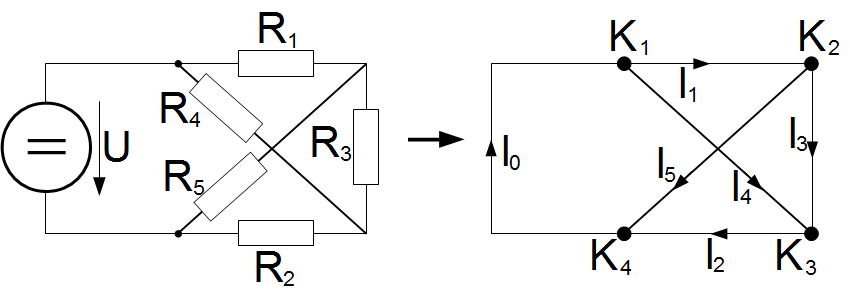
\includegraphics[scale=0.2]{source/graph.png}
					\item \textbf{Zählrichtung festlegen:} Für jeden Zweig die Richtung festlegen (muss konsequent beibehalten werden!).
					\item \textbf{Knotengleichungen aufstellen:} $k-1$ lin. un. Gleichu.:\\
					$\begin{array}{lllllllll}
						K_1: & I_0 & -I_1 & & & -I_4 & & = & 0 \\
						K_2: & & I_1 & & -I_3 & & -I_5 & = & 0 \\
						K_3: & & & -I_2 & +I_3 & +I_4 & & = & 0
					\end{array}$
					\item \textbf{Aufstellen der Maschengleichungen:}\\
					\#Maschengl.$=$\#Zweige$-$(\#Knoten$-1$)
				\end{enumerate}
				\begin{itemize}
					\item \textbf{Prinzip des vollständigen Baumes:}\\
					Ein vollständiger Baum ist eine Verbindung aller Knoten ohne einen geschlossenen Kreis. Danach muss jede Maschengleichung genau einen Zweig enthalten, der nicht zum vollständigen Baum gehört.
					\item \textbf{Prinzip der Auftrennung der Maschen:}\\
					Dabei wird nach dem Aufstellen einer Maschengl. Jeweils einer der verwendeten Zweige aufgetrennt und nie mehr verwendet.
				\end{itemize}
				\subsection{Superpositionsprinzip}
				Für jede Quelle das Netzwerk analysieren, die Anderen ausschalten, Resultate addieren.
				\begin{itemize}
					\item Spannungsquellen $\rightarrow$ Kurzschliessen
					\item Stromquellen $\rightarrow$ Leerlauf
				\end{itemize}				
				
			\section{Magnetostatik}
			\begin{itemize}
				\item \textbf{Magnetfeld:} Feldlinien von N nach S (innen S $\rightarrow$ N)\\
				Magnetfelder sind immer geschlossen.\\
				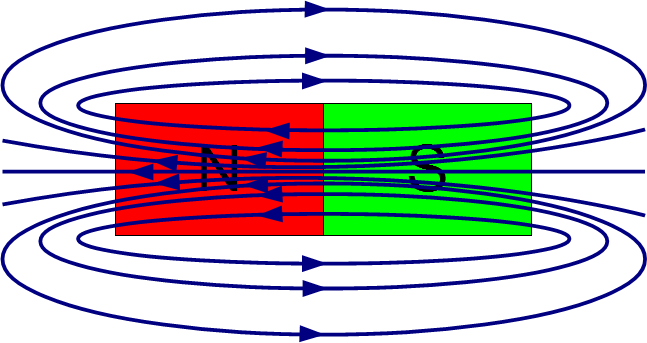
\includegraphics[scale=0.15]{source/magnet.png}\dis{1}
				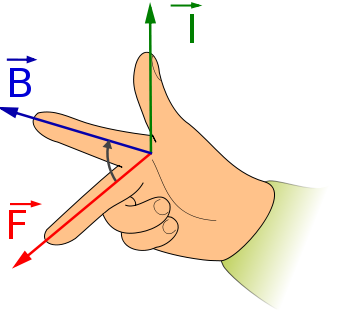
\includegraphics[scale=0.18]{source/rightHand.png}
				\item \textit{Mag. Flussdichte eines Leiters:} $\vec{B}=\frac{\mu_o}{2\pi}\frac{I}{\rho}, \, [T]=[\frac{Vs}{m^2}]$\\
				$\rho$ Abstand zum Leiter
				\item \textit{Mag. Feldstärke eines Leiters:} $\vec{H}=\frac{1}{\mu_0}\vec{B}=\frac{1}{2\pi}\frac{1}{\rho},[H]=\frac{A}{m}$
				\item \textit{Lorenzkraft (1-180):} $\vec{F}=q\vec{v}\times\vec{B}=I\vec{l}\times\vec{B}$
				\item \textit{F auf Ladung (1-183):} $\vec{F}_L=Q\cdot\vec{v}\times\vec{B}$\dis{0.2} $\vec{F}=Q\cdot(\vec{E}+\vec{v}\times\vec{B})$
			\end{itemize}
			\textbf{Analogie: Elektrisch, Magnetisch (1-209)}\\
			\begin{tabular}{|l|l|l|}
			\hline
			\textbf{Grösse} & \textbf{Elektrisch} & \textbf{Magnetisch} \\
			\hline
			Leitfähigkeit & $\kappa$ & $\mu$ \\
			\hline
			Widerstand & $R=\frac{1}{\kappa\cdot A}$ & $R_m=\frac{1}{\mu\cdot A}$ \\
			\hline
			Spannung & $U_{12}=\int_{P_1}^{P_2}\vec{E}\cdot d\vec{s}$ & \dis{-0.2}\begin{tabular}{l}
	$V_{m12}=\int_{P_1}^{P_2}\vec{H}\cdot d\vec{s}$ \\ $=R_{m12}\cdot\Phi_{12}$			
\end{tabular} \\
			\hline
			Strom/Fluss & \dis{-0.2}\begin{tabular}{l}
	$I=\iint_A\vec{J}\cdot d\vec{A}$ \\ $=\iint_A\vec{E}\cdot d\vec{A}$			
\end{tabular} & \dis{-0.2}\begin{tabular}{l}
	$\Phi=\iint_A\vec{B}\cdot d\vec{A}$ \\ $=\mu\iint_A\vec{H}\cdot d\vec{A}$			
\end{tabular} \\
			\hline
			Ohm. Gesetzt & $U=R\cdot I$ & $V_m=R_m\cdot\Phi$ \\
			\hline
			Maschengl. & $U_0=\sum_{Masche}RI$ & $\Theta=\sum_{Masche}R_m\Phi$ \\
			\hline
			Knotengl. & $\sum_{Knoten}I=0$ & $\sum_{Knoten}\Phi=0$ \\
			\hline
			
			\end{tabular}
			\begin{tabular}{|l|c|c|}
			\hline
			\textbf{Feldgrössen} & \dis{-0.2}\textbf{Elektrisch} & \dis{-0.2}\textbf{Magnetisch} \\
			\hline
			\dis{-0.2}Intensität/Wirkung(Kraft) & \dis{-0.2}$\vec{E}$ & \dis{-0.2}$\vec{B}=\mu\vec{H}$ \\
			\hline
			\dis{-0.2}Quantität/Ursache(Ladung) & \dis{-0.2}$\vec{D}=\varepsilon\vec{E}$ & \dis{-0.2}$\vec{H}$ \\
			\hline
			\end{tabular}
				\subsection{Oersted'sches Gesetz (Durchfl.satz)(1-187)}
				\eqbox{NI=\iint_A\vec{J}\cdot d\vec{A}=\Theta=\oint_{\partial A}\vec{H}\cdot d\vec{s}=\sum_k H_kl_k}\\
				$\Theta$ Durchflutung, $N$ Windungszahl\\
				Prinzip gilt insbesondere für $N=1$, sprich Einzelne Leiter
				\subsection{Verschiedene magnetische Komponenten}
				\begin{itemize}
					\item \textbf{$\infty$-langer Leiter (1-189):}
					$$\vec{H}(\rho)=\vec{e}_\varphi\cdot\frac{I}{2\pi}\begin{cases} \rho/R^2 & \rho \leq R \\ 1/\rho & \rho \geq R \end{cases}$$
					\item \textbf{Toroidspule (1-190):}
					$$NI=\Theta=\int_{0}^{2\pi}{\vec{e}_\varphi H_\varphi\rho}d\varphi=2\pi\rho H_\varphi(\rho)\rightarrow \vec{H}=\frac{NI}{2\pi\rho}\vec{e}_\varphi$$
					\item \textbf{Reluktanzmodell:} $H=\frac{NI}{l}\vec{e}_x$
					\item \textbf{Spannung über Spule:} Wenn sich die Spule bewegt, gilt nach dem Induktionsgesetz: $U_s=N\cdot\frac{d\Phi}{dt}$\\
					Dies vereinfacht sich zu: $U_s=l_s\cdot B\cdot v$ mit $l_s$: Leiterlänge im B-Feld, $v$: Geschwindigkeit mit der sich die Spule über den Kern bewegt.
				\end{itemize}
				\subsection{Reluktanzmodell (1-206)}
				\begin{itemize}
					\item \textbf{Magn. Spannung:} $V_m=\int_{P_1}^{P_2}{\vec{H}\cdot}d\vec{s}=\Theta=NI$\dis{0.2} $[\Theta]=A$
					\item \textbf{Magn. Strom:} $\Phi=\iint_A\vec{B}\cdot d\vec{A},$\dis{0.2} $[\Phi]=Vs=Wb$ (Weber)
					\item \textbf{Magn. Widerstand:} $R_m=\frac{l}{\mu A},$\dis{0.2} $[R_m]=\frac{1}{H}=\frac{A}{Vs}$
					\item \textbf{Magnetische spezifische Leitfähigkeit:} $\mu$
					\item \textbf{Magnetischer Leitwert:} $\Lambda_m=\frac{1}{R_m},$ \dis{0.2} $[\Lambda_m]=\frac{Vs}{A}$
					\item \textbf{Ohm'sches Gesetz:} $V_m=R_m\Phi,$\dis{0.2} $[V_m]=A$
				\end{itemize}
				\subsection{Magnetische Polarisation(1-199)}
				\textbf{Magnetische Polarisation:} $\vec{J_m}=\mu_0\mu_r\vec{H}-\mu_0\vec{H}$\\
				\textbf{Magnetisierung:} $\vec{M}=\mu_r\vec{H}-\vec{H}$\\
				\vspace{-0.5cm}
				\begingroup				
				\begin{wrapfigure}{r}{0.12\textwidth}
  				\begin{center}
   				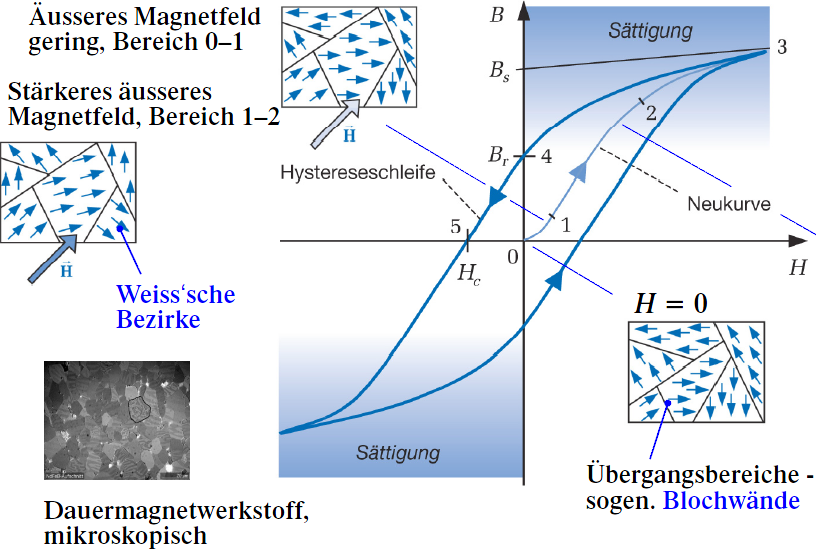
\includegraphics[scale=0.16]{source/hyst.png}
  				\end{center}
				\end{wrapfigure}
				
				\mbox{\textbf{Diamagnetismus:}}\\
				\mbox{Materialien, die das B-Feld}\\
				\mbox{schwächen, $\mu_r<1$}\\ \\
				\textbf{Paramagnetismus:}\\
				Materialien, die das B-Feld\\
				leicht stärken,  $\mu_r>1$\\\\
				\mbox{\textbf{Ferromagnetismus:}} \\
				Nebenan die Hysteresekurve\\
				eines Ferrit Materials\\
				\textit{Remanenz:} oberer Schnittpunkt mit y-Achse, $\mu_r>>1$, $\mu_r$ nicht konstant\\\\
				\textbf{Dauermagnete:} Ferromagnetische Stoffe im Remanenzzustand.
				\endgroup
				\subsection{Sprungstellen bei Materialübergängen (1-205)}
				\begin{itemize}
					\item \textit{Normalkomponenten:} \eqbox{B_{n1}=B_{n2}},\eqbox{\frac{H_{n1}}{H_{n2}}=\frac{\tan(\alpha_2)}{\tan(\alpha_1)}}
					\item \textit{Tangentialkomp.:} \eqbox{H_{t1}=H_{t2}},\eqbox{\frac{B_{t1}}{H_{t2}}=\frac{\mu_1}{\mu_2}=\frac{\tan(\alpha_1)}{\tan(\alpha_2)}}
				\end{itemize}
				\subsection{Induktivität (1-211)}
				$L=\frac{\Psi}{I}=\frac{N\Phi}{I}=\frac{N^2}{R_m},$\dis{0.3} $[L]=\frac{Vs}{A}=H$ (Henry)
				\begin{itemize}
					\item \textbf{$A_L$-Wert:} $L=N^2A_L=N^2\Lambda_m,$\dis{0.3} $A_L=\Lambda_m=\frac{1}{R_m}=[nH]$
					\item \textbf{Toroidspule:} $L=\frac{\Phi}{I}=\frac{N\Phi_A}{I}=N^2\frac{\mu H}{2\pi}\ln\left(\frac{r_{aussen}}{r_{innen}}\right)$
					\item \textbf{Luftspalt:} $L=N^2\frac{\mu_0\mu_{rel} A}{l_m\mu_{rel}d}\approx N^2\frac{\mu_0 A}{d}$\dis{0.2} $d$ Spaltgrösse
					\item \textbf{Kraft Magnetfeld:} $F_A=\frac{B^2}{2\mu_0}A$
				\end{itemize}
				\subsection{Induktion und Selbstinduktion(1-249)}
				\begin{itemize}
					\item \textbf{Induktionsgesetz:} $u(t)=-\frac{d\Phi}{dt}=-\frac{d}{dt}\iint_A\vec{B}\cdot d\vec{A}$
					\item \textbf{Selbstinduktion:} $u_L(t)=L\frac{di_L}{dt}$ (vgl. $i_C=C\frac{du_c}{dt}$)
					\item \textbf{Energie:} $W_m=W_L=\frac{1}{2}LI^2=\frac{1}{2}\Phi I=\iiint_V\frac{1}{2}\vec{B}\cdot\vec{H}dV$
				\end{itemize}
			
			\section{Allgemeines}
				\subsection{Einheiten}
				\vspace{-0.1cm}
				\begin{tabular}{|c|c|c|}
				\hline
				\textbf{} & \textbf{Einheit} & \textbf{Bedeutung} \\
				\hline
				$\vec{B}$ & $Vs/m^2$ & Magnetische Flussdichte \\
				\hline
				$B_r$ & $Vs/m^2$ & Remanenz \\
				\hline
				$C$ & $As/V=F$ & Kapazität \\
				\hline
				$\vec{D}$ & $As/m^2$ & Elektr. Flussdichte, el. Erregung \\
				\hline
				$\vec{E}$ & $V/m$ & Elektrische Feldstärke \\
				\hline
				G & $1/\Omega=A/V$ & Elektr. Leitwert \\
				\hline
				$\vec{H}$ & $A/m$ & Magn. Feldstärke \\
				\hline 
				$H_c$ & $A/m$ & Koerzitivfeldstärke \\
				\hline
				$I$ & $A$ & Gleichstrom \\
				\hline
			    $I_K$ & $A$ & Kurzschlussstrom \\
				\hline
				$i$ & $A$ & Zeitabhängiger Strom \\
				\hline
				$\vec{J}$ & $A/m^2$ & (räuml. vert.) Stromdichte \\
				\hline
				$\vec{J}$ & $Vs/m^2$ & Magn. Polarisation \\
				\hline
				$\vec{J}$ & $Vsm$ & Magn. Dipolmoment \\
				\hline
				$k$ & & Koppelfaktor \\
				\hline
				$L$ & $Vs/A$ & Induktivität \\
				\hline
				$\vec{M}$ & $A/m$ & Magnetisierung \\
				\hline
				$\vec{m}$ & $Am^2$ & Magnetisches Moment \\
				\hline
				$N$ & & Windungszahl \\
				\hline
				$P$ & $VA=W$ & Leistung \\
				\hline
				$p_V$ & $W/m^3$ & Verlustleistungsdichte \\
				\hline
				$\vec{P}$ & $As/m^2$ & Dielektr. Polarisation \\
				\hline
				$\vec{p}$ & $Asm$ & Elektr. Dipolmoment \\
				\hline
				$Q$ & $As=C$ & Ladung, Punktladung \\
				\hline
				$R$ & $V/A=\Omega$ & Ohmscher Widerstand \\
				\hline
				$R_m$ & $A/Vs$ & Magn. Widerstand \\
				\hline
				$U$ & $V$ & Gleichspannung \\
				\hline
				$u$ & $V$ & Zeitlich veränderliche Spannung \\
				\hline
				ü & & Übersetzungsverhältnis \\
				\hline
				$V_m$ & $A$ & Magnetische Spannung \\
				\hline
				$W$ & $VAs=J$ & Energie \\
				\hline
				$w$ & $WAs/m^3$ & Energiedichte \\
				\hline
				$\Phi$ & $Vs$ & Magnetischer Fluss \\
				\hline
				$\Lambda_m$ & $Vs/A$ & Magnetischer Leitwert \\
				\hline
				$\Theta$ & $A$ & Durchflutung \\
				\hline
				$\Psi$ & $As$ & Elektr. Fluss \\
				\hline
				$\alpha$ & $1/K$ & Temperaturkoeffizient \\
				\hline
				$\chi$ & & Dielekt. \& magn. Suszeptibilität \\
				\hline
				$\varepsilon$ & $As/Vm$ & Dielektrizitätskonstante \\
				\hline
				$\varepsilon_r$ & & Dielektrizitätszahl \\
				\hline
				$\varphi$ &  & Phasenwinkel \\
				\hline
				$\varphi_e$ & $V$ & Elektrostatisches Potential \\
				\hline
				$\eta$ & & Wirkungsgrad \\
				\hline
				$\kappa$ & $A/Vm$ & Spezifische Leitfähigkeit \\
				\hline
				$\lambda$ & $As/m$ & Linienladungsdichte \\
				\hline
				$\mu$ & $Vs/Am$ & Permeabilität \\
				\hline
				$\mu_e$ & $m^2/Vs$ & Beweglichkeit der Ladungsträger \\
				\hline
				$\rho$ & $As/m^3$ & Raumladungsdichte \\
				\hline
				$\rho_R$ & $Vm/A$ & Spezifischer Widerstand \\
				\hline
				$\sigma$ & $As/m^2$ & Flächenladung \\
				\hline
				$\sigma$ & & Streugrad \\
				\hline
				$\omega$ & $1/s\cdot 2\pi$ & Kreisfrequenz \\
				\hline
				\end{tabular}											
    \end{multicols*}
\setcounter{secnumdepth}{2}
\end{document}
